\documentclass[12pt]{article}
\usepackage[margin=1in]{geometry}
\usepackage{amsmath, amsthm, amssymb, mathtools, mathrsfs}
\usepackage{enumitem, graphicx, hyperref, booktabs, array}
\usepackage[mathscr]{euscript}
\usepackage[T1]{fontenc}
\usepackage{microtype}
\usepackage{tikz}
\usetikzlibrary{shapes,arrows,positioning}
\hypersetup{colorlinks=true, linkcolor=blue, citecolor=red}

% Mathematical operators and notation
\DeclareMathOperator{\argmin}{arg\,min}
\DeclareMathOperator{\argmax}{arg\,max}
\DeclareMathOperator{\sign}{sign}
\DeclareMathOperator{\diag}{diag}
\DeclareMathOperator{\rank}{rank}
\DeclareMathOperator{\card}{card}
\renewcommand{\vec}[1]{\mathbf{#1}}
\newcommand{\norm}[1]{\left\lVert #1 \right\rVert}
\newcommand{\abs}[1]{\left| #1 \right|}
\newcommand{\R}{\mathbb{R}}
\newcommand{\E}{\mathbb{E}}

% Theorem environments
\theoremstyle{definition}
\newtheorem{definition}{Definition}[section]
\newtheorem{theorem}{Theorem}[section]
\newtheorem{lemma}[theorem]{Lemma}
\newtheorem{corollary}[theorem]{Corollary}
\newtheorem{proposition}[theorem]{Proposition}
\newtheorem{example}{Example}[section]
\newtheorem{remark}{Remark}[section]
\newtheorem{algorithm}{Algorithm}[section]

\title{Robust Model Fitting in Computer Vision: Theory and Algorithms}
\author{Lecture Notes}
\date{\today}

\begin{document}

\maketitle

\begin{abstract}
    These notes provide a comprehensive treatment of robust model fitting techniques in computer vision, with particular emphasis on geometric primitives such as lines and circles. We explore both classical least squares approaches and modern robust methods including RANSAC and its variants. The mathematical foundations are developed rigorously, from the Direct Linear Transformation (DLT) algorithm to M-estimators and greedy consensus maximization strategies.
\end{abstract}

\tableofcontents
\newpage

%=====================================
\section{Introduction to Robust Fitting}
%=====================================

\subsection{Motivation and Problem Formulation}

The problem of \textit{robust model fitting} arises ubiquitously in computer vision applications where we must estimate analytical expressions derived from geometric constraints in the presence of outliers. Unlike standard noise, outliers represent data points that significantly deviate from the expected model with statistical characteristics that are fundamentally different from the inlier distribution.

\begin{definition}[Robust Fitting Problem]
    Given a set of observations $\mathcal{D} = \{(\vec{x}_i, y_i)\}_{i=1}^n$ where $\vec{x}_i \in \R^d$ and $y_i \in \R$, the robust fitting problem seeks to estimate parameters $\vec{\theta} \in \R^p$ of a model $f(\vec{x}; \vec{\theta})$ such that:
    \begin{equation}
        \vec{\theta}^* = \argmin_{\vec{\theta}} \sum_{i=1}^n \rho(r_i(\vec{\theta}))
    \end{equation}
    where $r_i(\vec{\theta}) = y_i - f(\vec{x}_i; \vec{\theta})$ is the residual and $\rho: \R \to \R^+$ is a robust loss function.
\end{definition}

The choice of $\rho$ fundamentally determines the robustness properties of the estimator. Classical least squares uses $\rho(r) = r^2$, which, as we shall demonstrate, lacks robustness to outliers.

\subsection{Applications in Computer Vision}

Robust fitting finds applications across numerous computer vision tasks:

\begin{enumerate}[label=(\roman*)]
    \item \textbf{Sports Analytics}: Fitting lines of a soccer field from camera views enables real-time player tracking and tactical analysis. This requires fitting multiple line models simultaneously while handling occlusions and perspective distortions.

    \item \textbf{Document Rectification}: Mobile document scanning applications detect quadrilaterals by fitting four line equations, then compute a homography to rectify the perspective distortion.

    \item \textbf{3D Reconstruction}: Establishing point correspondences between images requires robust estimation of the fundamental matrix $\vec{F} \in \R^{3 \times 3}$ relating epipolar geometry.

    \item \textbf{Object Detection}: Template matching and object localization often involve fitting geometric primitives to edge features extracted from images.
\end{enumerate}

% NOTE: Adding conceptual diagram of robust fitting scenarios
\begin{figure}[h]
    \centering
    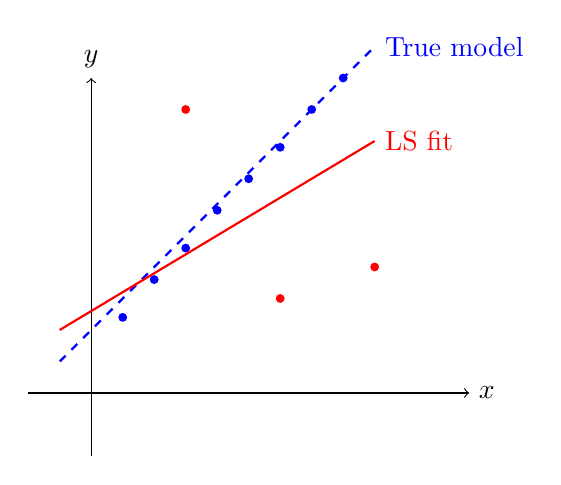
\begin{tikzpicture}[scale=0.8]
        % Coordinate system
        \draw[->] (-1,0) -- (6,0) node[right] {$x$};
        \draw[->] (0,-1) -- (0,5) node[above] {$y$};
        % Inliers
        \foreach \x/\y in {0.5/1.2, 1/1.8, 1.5/2.3, 2/2.9, 2.5/3.4, 3/3.9, 3.5/4.5, 4/5.0} {
                \fill[blue] (\x,\y) circle (2pt);
            }
        % Outliers
        \foreach \x/\y in {1.5/4.5, 3/1.5, 4.5/2.0} {
                \fill[red] (\x,\y) circle (2pt);
            }
        % True line
        \draw[thick, blue, dashed] (-0.5,0.5) -- (4.5,5.5) node[right] {True model};
        % Least squares line (affected by outliers)
        \draw[thick, red] (-0.5,1.0) -- (4.5,4.0) node[right] {LS fit};
    \end{tikzpicture}
    \caption{Illustration of outlier influence on least squares fitting}
\end{figure}

\newpage
%=====================================
\section{Classical Least Squares Approaches}
%=====================================

\subsection{Ordinary Least Squares for Line Fitting}

We begin with the fundamental problem of fitting a straight line to a set of 2D points. The parametric form of a line is:
\begin{equation}
    y = mx + b
\end{equation}
where $m$ is the slope and $b$ is the y-intercept. Given observations $\{(x_i, y_i)\}_{i=1}^n$, ordinary least squares (OLS) seeks:

\begin{equation}
    (m^*, b^*) = \argmin_{m,b} \sum_{i=1}^n (y_i - mx_i - b)^2
\end{equation}

\subsubsection{Matrix Formulation and Solution}

Define the design matrix $\vec{A} \in \R^{n \times 2}$ and parameter vector $\vec{\theta} \in \R^2$:
\begin{equation}
    \vec{A} = \begin{bmatrix}
        x_1    & 1      \\
        x_2    & 1      \\
        \vdots & \vdots \\
        x_n    & 1
    \end{bmatrix}, \quad
    \vec{\theta} = \begin{bmatrix}
        m \\ b
    \end{bmatrix}, \quad
    \vec{y} = \begin{bmatrix}
        y_1 \\ y_2 \\ \vdots \\ y_n
    \end{bmatrix}
\end{equation}

The optimization problem becomes:
\begin{equation}
    \vec{\theta}^* = \argmin_{\vec{\theta}} \norm{\vec{y} - \vec{A}\vec{\theta}}_2^2
\end{equation}

\begin{theorem}[Normal Equations]
    The optimal parameters for the least squares problem are given by:
    \begin{equation}
        \vec{\theta}^* = (\vec{A}^T\vec{A})^{-1}\vec{A}^T\vec{y}
    \end{equation}
    provided that $\vec{A}^T\vec{A}$ is invertible (i.e., $\rank(\vec{A}) = 2$).
\end{theorem}

\begin{proof}
    Taking the gradient of the objective function:
    \begin{align}
        \nabla_{\vec{\theta}} \norm{\vec{y} - \vec{A}\vec{\theta}}_2^2 & = \nabla_{\vec{\theta}} (\vec{y} - \vec{A}\vec{\theta})^T(\vec{y} - \vec{A}\vec{\theta}) \\
                                                                       & = -2\vec{A}^T(\vec{y} - \vec{A}\vec{\theta})
    \end{align}
    Setting the gradient to zero yields the normal equations:
    \begin{equation}
        \vec{A}^T\vec{A}\vec{\theta} = \vec{A}^T\vec{y}
    \end{equation}
    When $\vec{A}^T\vec{A}$ is invertible, we obtain the closed-form solution.
\end{proof}

\subsection{Limitations of Vertical Distance Minimization}

The ordinary least squares approach measures error along the vertical axis, which introduces several fundamental limitations:

\begin{enumerate}
    \item \textbf{Inability to fit vertical lines}: When the line approaches vertical ($m \to \infty$), the formulation breaks down as we cannot express $x$ as a function of $y$.

    \item \textbf{Asymmetric treatment of variables}: The choice of dependent vs. independent variable artificially privileges one coordinate axis.

    \item \textbf{Scale dependency}: The error metric depends on the coordinate system orientation.
\end{enumerate}

\newpage
%=====================================
\section{The Direct Linear Transformation (DLT) Algorithm}
%=====================================

\subsection{Implicit Line Representation}

To overcome the limitations of parametric representations, we adopt the implicit form:
\begin{equation}
    ax + by + c = 0
\end{equation}
where $(a, b, c) \in \R^3$ are the line parameters. This representation elegantly handles all line orientations, including vertical lines (where $b = 0$).

\begin{remark}
    The implicit representation introduces a scale ambiguity: the lines defined by $(a, b, c)$ and $(\lambda a, \lambda b, \lambda c)$ for any $\lambda \neq 0$ are identical. This necessitates a normalization constraint.
\end{remark}

\subsection{Algebraic Error Minimization}

Rather than minimizing geometric distance (which leads to nonlinear optimization), we minimize the \textit{algebraic error}:

\begin{definition}[Algebraic Error]
    For a point $(x_i, y_i)$ and line parameters $\vec{\theta} = [a, b, c]^T$, the algebraic error is:
    \begin{equation}
        r_i^{alg}(\vec{\theta}) = ax_i + by_i + c
    \end{equation}
\end{definition}

% NOTE: Geometric vs algebraic error comparison
The relationship between algebraic and geometric errors is:
\begin{equation}
    r_i^{geom}(\vec{\theta}) = \frac{\abs{ax_i + by_i + c}}{\sqrt{a^2 + b^2}} = \frac{\abs{r_i^{alg}(\vec{\theta})}}{\sqrt{a^2 + b^2}}
\end{equation}

\subsection{Constrained Least Squares Formulation}

The DLT problem is formulated as:
\begin{equation}
    \vec{\theta}^* = \argmin_{\vec{\theta}} \norm{\vec{A}\vec{\theta}}_2^2 \quad \text{subject to} \quad \norm{\vec{\theta}}_2 = 1
\end{equation}
where the design matrix is:
\begin{equation}
    \vec{A} = \begin{bmatrix}
        x_1    & y_1    & 1      \\
        x_2    & y_2    & 1      \\
        \vdots & \vdots & \vdots \\
        x_n    & y_n    & 1
    \end{bmatrix} \in \R^{n \times 3}
\end{equation}

\begin{theorem}[DLT Solution via SVD] \label{thm:dlt}
    Let $\vec{A} = \vec{U}\vec{\Sigma}\vec{V}^T$ be the singular value decomposition of $\vec{A}$, where:
    \begin{itemize}
        \item $\vec{U} \in \R^{n \times n}$ and $\vec{V} \in \R^{3 \times 3}$ are orthogonal matrices
        \item $\vec{\Sigma} = \diag(\sigma_1, \sigma_2, \sigma_3)$ with $\sigma_1 \geq \sigma_2 \geq \sigma_3 \geq 0$
    \end{itemize}
    Then the optimal solution is $\vec{\theta}^* = \vec{v}_3$, the last column of $\vec{V}$.
\end{theorem}

\begin{proof}
    Using the orthogonality of $\vec{U}$ and the substitution $\vec{w} = \vec{V}^T\vec{\theta}$:
    \begin{align}
        \norm{\vec{A}\vec{\theta}}_2^2 & = \norm{\vec{U}\vec{\Sigma}\vec{V}^T\vec{\theta}}_2^2                               \\
                                       & = \norm{\vec{\Sigma}\vec{V}^T\vec{\theta}}_2^2 \quad \text{(orthogonal invariance)} \\
                                       & = \norm{\vec{\Sigma}\vec{w}}_2^2 = \sum_{i=1}^3 \sigma_i^2 w_i^2
    \end{align}

    Since $\norm{\vec{\theta}}_2 = \norm{\vec{w}}_2 = 1$, minimizing the objective requires placing all weight on the smallest singular value:
    \begin{equation}
        \vec{w}^* = [0, 0, 1]^T \implies \vec{\theta}^* = \vec{V}\vec{w}^* = \vec{v}_3
    \end{equation}
\end{proof}

\subsection{Preconditioning for Numerical Stability}

Numerical conditioning is crucial for stable DLT computation, especially when dealing with higher-order geometric entities.

\begin{algorithm}[Normalized DLT]
    \begin{enumerate}
        \item Compute data centroid and scale:
              \begin{equation}
                  \bar{x} = \frac{1}{n}\sum_{i=1}^n x_i, \quad \bar{y} = \frac{1}{n}\sum_{i=1}^n y_i
              \end{equation}

        \item Apply normalization transformation:
              \begin{equation}
                  \vec{T} = \begin{bmatrix}
                      s_x & 0   & -s_x\bar{x} \\
                      0   & s_y & -s_y\bar{y} \\
                      0   & 0   & 1
                  \end{bmatrix}
              \end{equation}
              where $s_x$ and $s_y$ are chosen such that the normalized data has unit variance.

        \item Solve DLT for normalized points: $\tilde{\vec{\theta}}^* = \text{DLT}(\{\vec{T}\vec{p}_i\})$

        \item Denormalize the solution: $\vec{\theta}^* = \vec{T}^T\tilde{\vec{\theta}}^*$
    \end{enumerate}
\end{algorithm}

\newpage
%=====================================
\section{Robust Estimation Methods}
%=====================================

\subsection{The Breakdown Point and Robustness}

\begin{definition}[Breakdown Point]
    The breakdown point $\epsilon^*$ of an estimator is the largest fraction of arbitrarily corrupted observations that the estimator can handle while still producing a bounded estimate close to the true value.
\end{definition}

For ordinary least squares, the breakdown point is $\epsilon^* = 0$, meaning a single outlier with sufficient leverage can arbitrarily corrupt the estimate. This motivates the development of robust alternatives.

\subsection{M-Estimators}

M-estimators generalize maximum likelihood estimation by replacing the squared loss with robust alternatives:

\begin{equation}
    \vec{\theta}^* = \argmin_{\vec{\theta}} \sum_{i=1}^n \rho(r_i(\vec{\theta}))
\end{equation}

Common choices for $\rho$ include:

\begin{table}[h]
    \centering
    \begin{tabular}{lcc}
        \toprule
        Name                & $\rho(r)$                                                                                          & Influence Function $\psi(r) = \rho'(r)$                                        \\
        \midrule
        L2 (Least Squares)  & $r^2$                                                                                              & $2r$                                                                           \\
        L1 (Least Absolute) & $\abs{r}$                                                                                          & $\sign(r)$                                                                     \\
        Huber               & $\begin{cases} r^2/2 & \abs{r} \leq k \\ k\abs{r} - k^2/2 & \abs{r} > k \end{cases}$               & $\begin{cases} r & \abs{r} \leq k \\ k\sign(r) & \abs{r} > k \end{cases}$      \\
        Tukey's Bisquare    & $\begin{cases} \frac{k^2}{6}[1-(1-r^2/k^2)^3] & \abs{r} \leq k \\ k^2/6 & \abs{r} > k \end{cases}$ & $\begin{cases} r(1-r^2/k^2)^2 & \abs{r} \leq k \\ 0 & \abs{r} > k \end{cases}$ \\
        \bottomrule
    \end{tabular}
    \caption{Common M-estimator loss functions and their derivatives}
\end{table}

\subsection{RANSAC: Random Sample Consensus}

RANSAC takes a fundamentally different approach by explicitly modeling the presence of outliers through a consensus framework.

\subsubsection{The Consensus Set}

\begin{definition}[Consensus Set]
    Given parameters $\vec{\theta}$ and threshold $\epsilon$, the consensus set is:
    \begin{equation}
        \mathcal{C}(\vec{\theta}) = \{i : \abs{r_i(\vec{\theta})} \leq \epsilon\}
    \end{equation}
\end{definition}

RANSAC maximizes the cardinality of the consensus set:
\begin{equation}
    \vec{\theta}^* = \argmax_{\vec{\theta}} \abs{\mathcal{C}(\vec{\theta})}
\end{equation}

\subsubsection{The RANSAC Algorithm}

\begin{algorithm}[RANSAC] \label{alg:ransac}
    \textbf{Input:} Data points $\mathcal{D}$, inlier threshold $\epsilon$, confidence $p$ \\
    \textbf{Output:} Model parameters $\vec{\theta}^*$

    \begin{enumerate}
        \item Initialize: $\mathcal{C}^* = \emptyset$, $k = 0$

        \item \textbf{while} $k < N$ \textbf{do}:
              \begin{enumerate}[label=(\alph*)]
                  \item Randomly sample minimal set $\mathcal{S} \subset \mathcal{D}$ with $\abs{\mathcal{S}} = m$
                  \item Fit model: $\vec{\theta}_k = \text{FitModel}(\mathcal{S})$
                  \item Evaluate consensus: $\mathcal{C}_k = \{i : \abs{r_i(\vec{\theta}_k)} \leq \epsilon\}$
                  \item \textbf{if} $\abs{\mathcal{C}_k} > \abs{\mathcal{C}^*}$ \textbf{then} $\mathcal{C}^* = \mathcal{C}_k$, $\vec{\theta}^* = \vec{\theta}_k$
              \end{enumerate}

        \item Refine: $\vec{\theta}^* = \text{LeastSquares}(\mathcal{C}^*)$
    \end{enumerate}
\end{algorithm}

\subsubsection{Determining the Number of Iterations}

The number of iterations $N$ is determined probabilistically to ensure finding at least one outlier-free sample with confidence $p$:

\begin{theorem}[RANSAC Iteration Count]
    Given inlier ratio $w$ and desired confidence $p$, the required number of iterations is:
    \begin{equation}
        N = \frac{\log(1-p)}{\log(1-w^m)}
    \end{equation}
    where $m$ is the minimal sample size.
\end{theorem}

\begin{proof}
    The probability of selecting an all-inlier minimal sample is $w^m$. The probability of failing to select such a sample in $N$ attempts is $(1-w^m)^N$. Setting this equal to $1-p$ and solving for $N$ yields the result.
\end{proof}

% NOTE: Practical values for different scenarios
\begin{example}
    For line fitting ($m=2$) with 50\% inliers ($w=0.5$) and 99\% confidence ($p=0.99$):
    \begin{equation}
        N = \frac{\log(0.01)}{\log(1-0.5^2)} = \frac{\log(0.01)}{\log(0.75)} \approx 17
    \end{equation}
\end{example}

\subsection{MSAC and MLESAC Variants}

\subsubsection{MSAC: M-estimator Sample Consensus}

MSAC refines RANSAC by considering the magnitude of residuals within the inlier band:

\begin{equation}
    L_{MSAC}(\vec{\theta}) = \sum_{i=1}^n \min(\abs{r_i(\vec{\theta})}, \epsilon)
\end{equation}

This formulation corresponds to a truncated L1 loss, providing better discrimination between competing models with similar consensus set sizes.

\subsubsection{MLESAC: Maximum Likelihood Sample Consensus}

MLESAC models the error distribution explicitly as a mixture:
\begin{equation}
    p(r_i) = \gamma \mathcal{N}(0, \sigma^2) + (1-\gamma) \mathcal{U}(-v, v)
\end{equation}
where $\gamma$ is the inlier ratio, and maximizes the likelihood of the observed residuals.

\newpage
%=====================================
\section{Advanced Topics and Applications}
%=====================================

\subsection{Multi-Model Fitting}

Real-world scenarios often require fitting multiple models simultaneously. Consider detecting multiple lines in an edge map or multiple planes in a point cloud.

\begin{definition}[Multi-Model Fitting Problem]
    Given data $\mathcal{D}$, find models $\{\vec{\theta}_j\}_{j=1}^K$ and assignments $\{z_i\}_{i=1}^n$ where $z_i \in \{1, \ldots, K, K+1\}$ (with $K+1$ denoting outliers) that minimize:
    \begin{equation}
        \sum_{j=1}^K \sum_{i: z_i = j} \rho(r_i(\vec{\theta}_j)) + \lambda \cdot \abs{\{i: z_i = K+1\}}
    \end{equation}
\end{definition}

\subsection{Adaptive Threshold Selection}

The inlier threshold $\epsilon$ critically affects RANSAC performance. Adaptive methods estimate $\epsilon$ from the data:

\begin{algorithm}[Adaptive RANSAC]
    \begin{enumerate}
        \item Initial fit using conservative $\epsilon_0$
        \item Estimate noise level from inlier residuals:
              \begin{equation}
                  \hat{\sigma} = \text{MAD}(\{r_i : i \in \mathcal{C}^*\}) / 0.6745
              \end{equation}
              where MAD is the median absolute deviation.
        \item Update threshold: $\epsilon = k\hat{\sigma}$ (typically $k \in [2.5, 3]$)
        \item Iterate until convergence
    \end{enumerate}
\end{algorithm}

\subsection{Geometric Constraints and Manifold Fitting}

When fitting models with geometric constraints (e.g., orthogonal lines, concentric circles), the parameter space forms a manifold. The optimization becomes:
\begin{equation}
    \vec{\theta}^* = \argmin_{\vec{\theta} \in \mathcal{M}} \sum_{i=1}^n \rho(r_i(\vec{\theta}))
\end{equation}
where $\mathcal{M}$ represents the constraint manifold.

\begin{example}[Orthogonal Line Pairs]
    For two orthogonal lines with parameters $\vec{\theta}_1 = [a_1, b_1, c_1]^T$ and $\vec{\theta}_2 = [a_2, b_2, c_2]^T$, the constraint is:
    \begin{equation}
        a_1 a_2 + b_1 b_2 = 0
    \end{equation}
    This reduces the degrees of freedom from 6 to 5.
\end{example}

\subsection{Performance Analysis and Guarantees}

\begin{theorem}[RANSAC Success Probability]
    The probability that RANSAC finds the correct model after $N$ iterations is:
    \begin{equation}
        P_{success} = 1 - (1 - w^m)^N
    \end{equation}
    where the bound is tight when outliers are uniformly distributed.
\end{theorem}

For structured outliers (e.g., points from another model), the actual performance can be significantly better than this worst-case bound.

\newpage
%=====================================
\section{Implementation Considerations}
%=====================================

\subsection{Efficient Sampling Strategies}

\subsubsection{Guided Sampling}
Rather than uniform random sampling, guided sampling exploits prior information:
\begin{itemize}
    \item \textbf{Proximity-based}: Sample points that are spatially close
    \item \textbf{Feature-based}: Use appearance similarity to guide sampling
    \item \textbf{Progressive sampling}: Adaptively update sampling distribution based on previous iterations
\end{itemize}

\subsubsection{Deterministic Sampling}
For small datasets, exhaustive evaluation of all $\binom{n}{m}$ minimal samples may be feasible and guarantees finding the optimal solution.

\subsection{Parallel Implementation}

RANSAC's iterations are inherently parallel, making GPU implementation attractive:

\begin{algorithm}[Parallel RANSAC]
    \begin{enumerate}
        \item Distribute iterations across $P$ processors
        \item Each processor maintains local best model
        \item Global reduction to find overall best model
        \item Load balancing through dynamic work distribution
    \end{enumerate}
\end{algorithm}

\subsection{Degeneracy Detection}

Degenerate configurations (e.g., collinear points for circle fitting) must be detected and rejected:

\begin{definition}[Degenerate Configuration]
    A minimal sample $\mathcal{S}$ is degenerate if it does not uniquely determine the model parameters, i.e., $\dim(\text{null}(\vec{A}_\mathcal{S})) > 1$.
\end{definition}

\subsection{Quality Metrics}

Beyond consensus set size, additional metrics help evaluate model quality:

\begin{enumerate}
    \item \textbf{Residual statistics}: Mean, median, and variance of inlier residuals
    \item \textbf{Distribution tests}: Kolmogorov-Smirnov test for residual normality
    \item \textbf{Geometric consistency}: Preservation of known geometric relationships
    \item \textbf{Cross-validation}: Performance on held-out data
\end{enumerate}
\end{document}